\documentclass{beamer}					% Document class

\mode<presentation>
{
  \usetheme{default}                    % Set theme
  \usecolortheme{default}               % Set colors
  \usefonttheme{default}                % Set font theme
  \setbeamertemplate{caption}[numbered] % Set caption to be numbered
}

\usepackage{graphicx}  % For including figures
\usepackage{booktabs}  % For table rules
\usepackage{hyperref}  % For cross-referencing

\title{My Biography}  % Presentation title
\author{Frank Kusi Agyemang}                              % Presentation author
\institute{University of Nebraska-Lincoln}                  % Author affiliation
\date{\today}                                    % Today's date

% This creates a bibliography file with the same name as the main file.
% Mostly, it allows us to have only one text file to lug around.
\begin{filecontents}{\jobname.bib}
	title = {Fuck {Nuance}},
	volume = {35},
	doi = {10.1177/0735275117709046},
	number = {2},
	journal = {Sociological Theory},
	author = {Healy, Kieran},
	month = jun,
	year = {2017},
	pages = {118--127}
}
	title = {Everything is awesome: Don't forget the {Lego}},
	volume = {55},
	doi = {10.1111/jpc.14309},
	number = {8},
	journal = {Journal of Paediatrics and Child Health},
	author = {Tagg, Andrew and Roland, Damian and Leo, Grace SY and Knight, Katie and Goldstein, Henry and Davis, Tessa},
	year = {2019},
	pages = {921--923},
}
\end{filecontents}


\usepackage{Sweave}
\begin{document}
\Sconcordance{concordance:beamer-demo.tex:beamer-demo.Rnw:%
1 100 1 49 0 15 1 8 0 3 1}



\begin{frame}
  \titlepage 
\end{frame}


\begin{frame}{Outline}
  \tableofcontents 
\end{frame}

\section{Background}

\begin{frame}{About Me}
	My name is Frank Kusi Agyemang. I am from Ghana and currently a graduate student at the University of Nebraska-Lincoln, pursuing a Master of Science degree in Statistics. I am 23yrs old. I was born in Kumasi, the second largest city in Ghana. Additional things that I would add are my hobbies. Good food and good music.
\end{frame}

\section{Favorite Pets}

\begin{frame}{Favorite Pets}
\begin{itemize}
        \item Penguins
	\end{itemize}
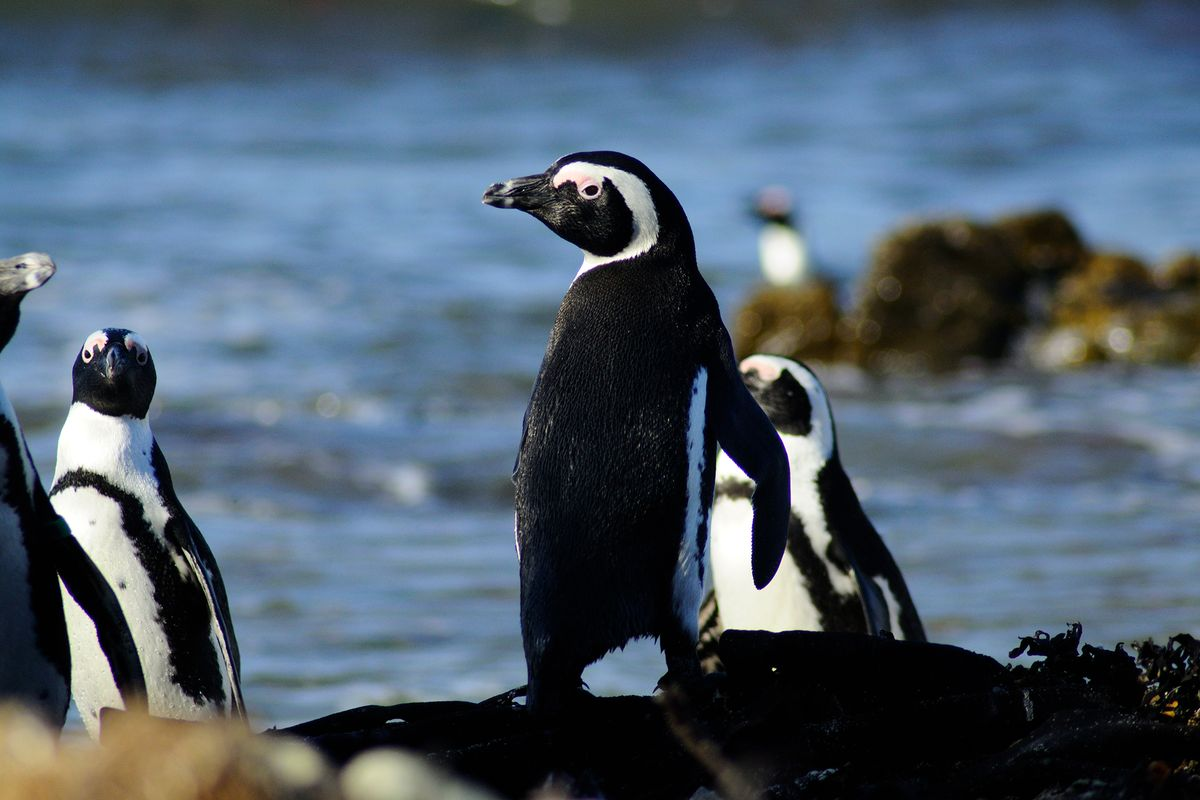
\includegraphics[scale=0.6]{penguin.png}
\end{frame}


\begin{frame}
\begin{itemize}
		\item Parrots
\end{itemize}
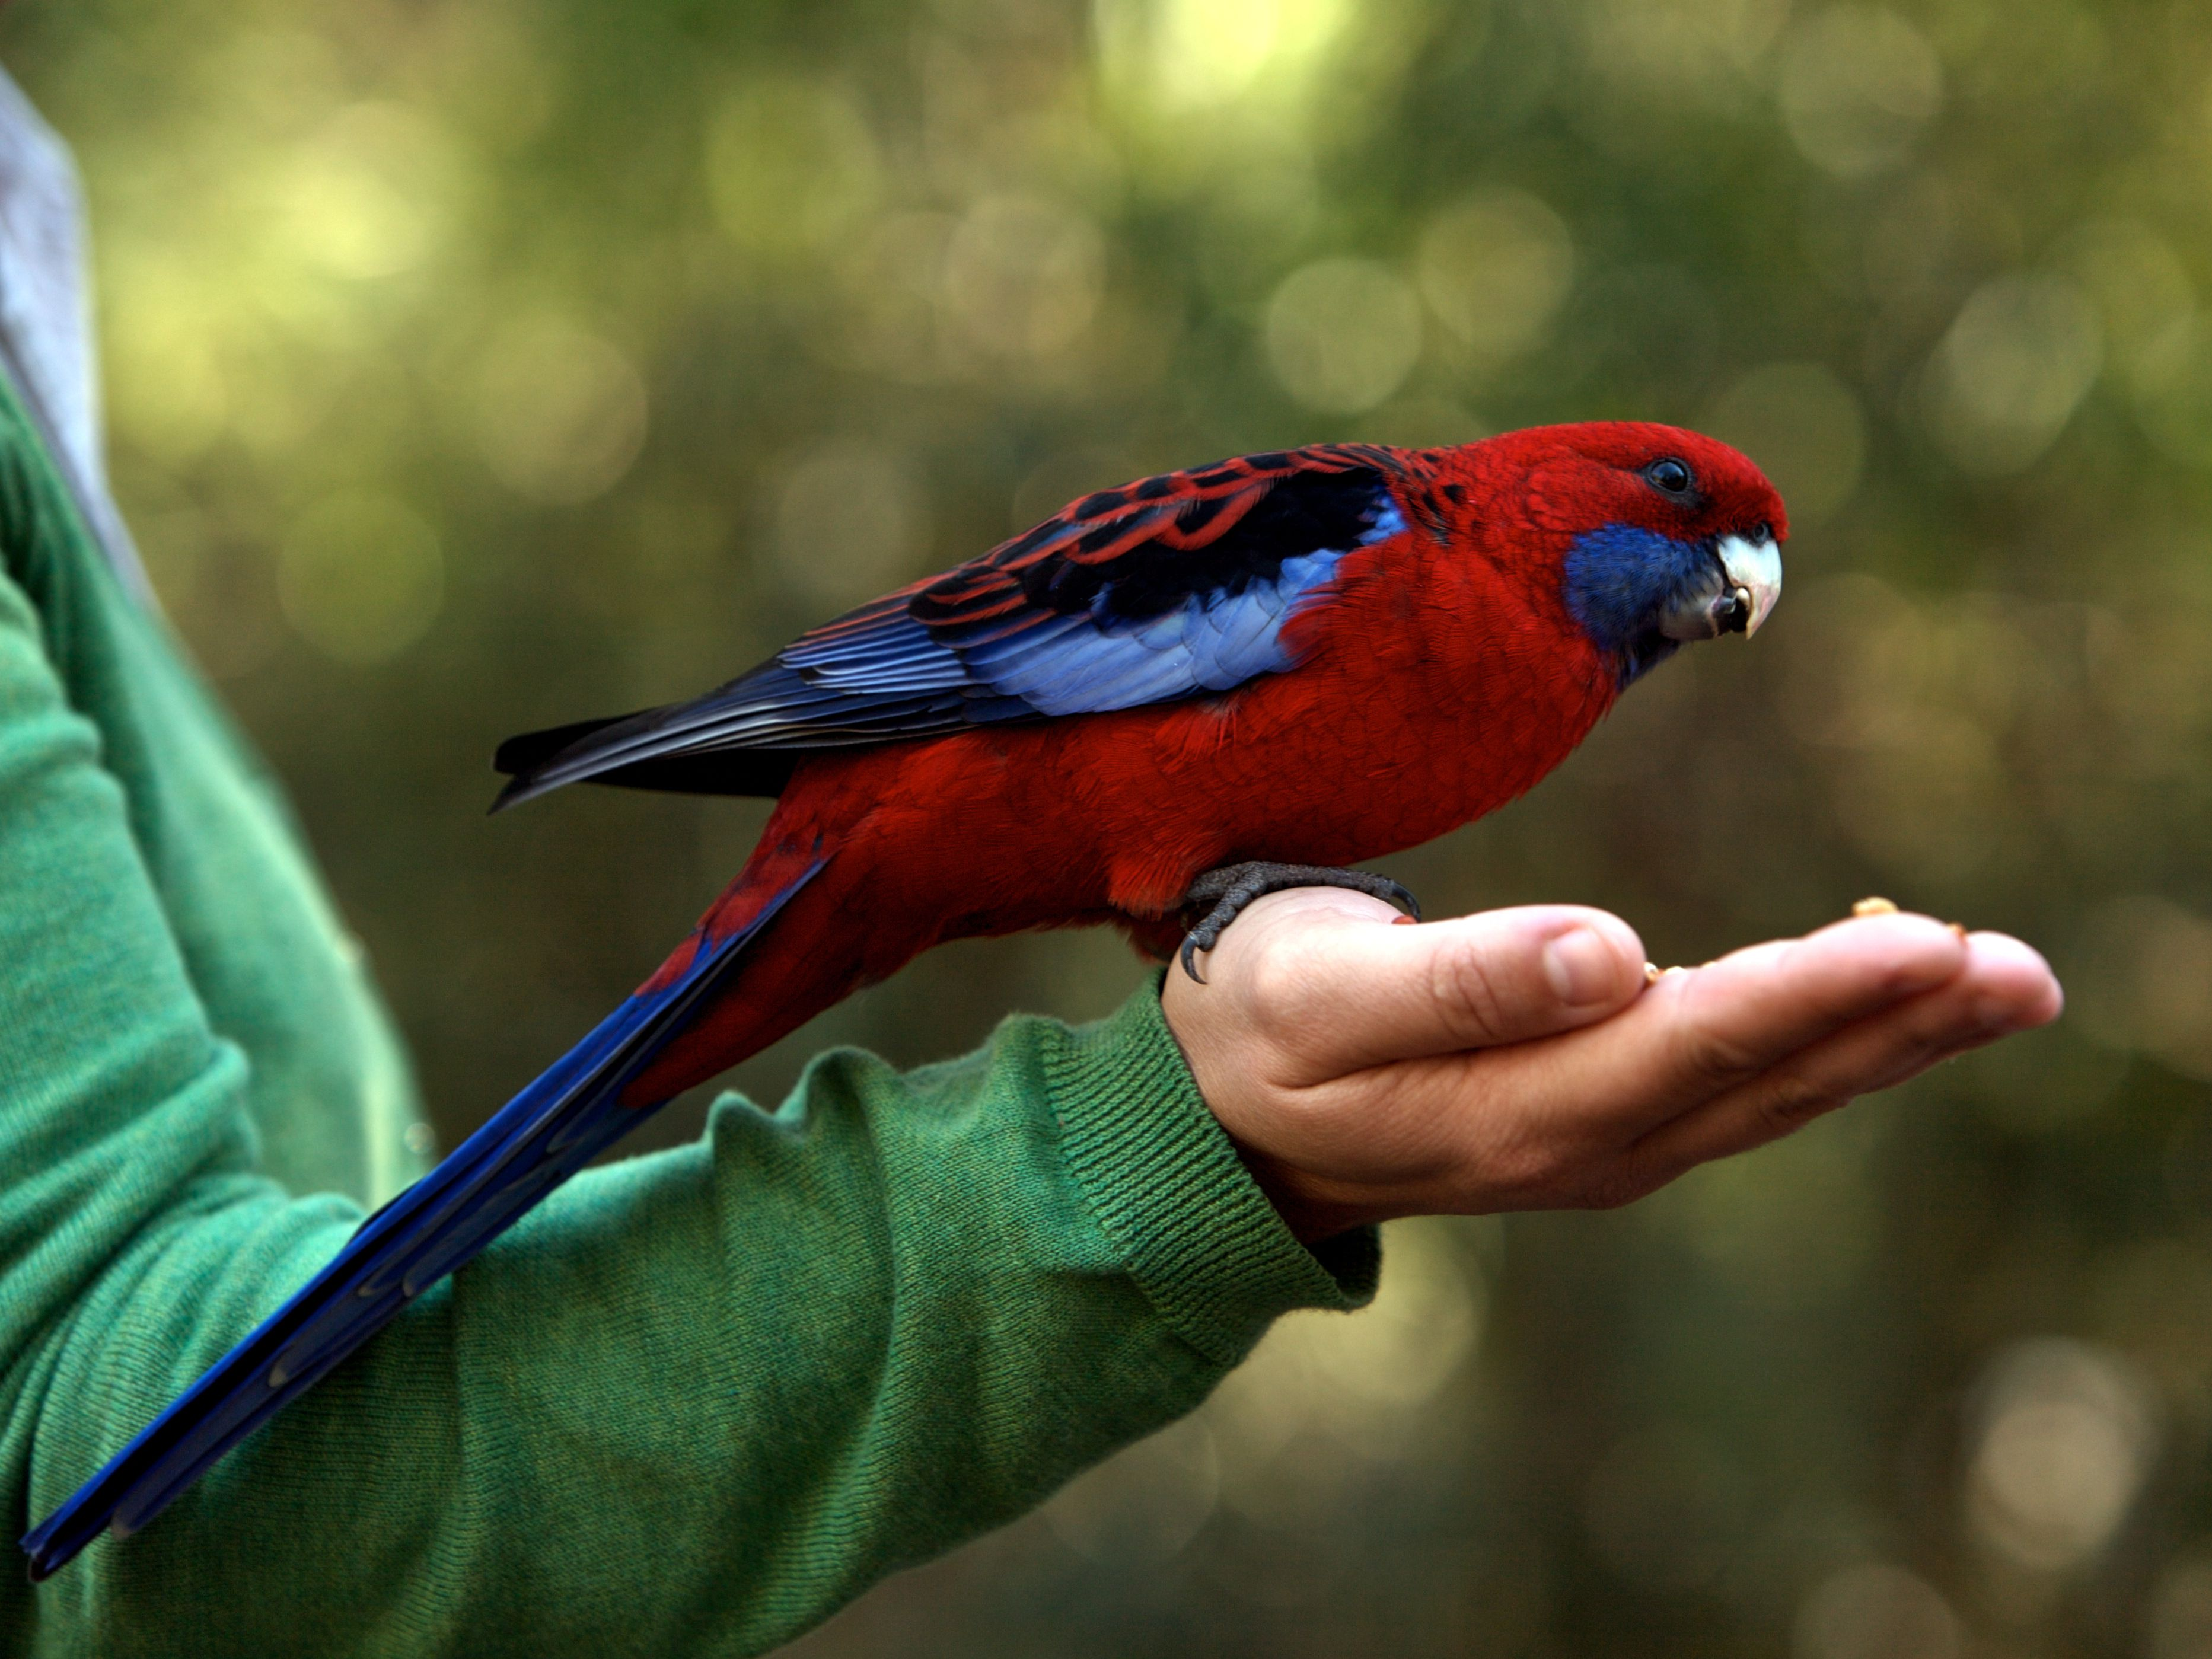
\includegraphics[scale=0.7]{parrots.png}

\end{frame}

\section{Graphs}






% Adding the option 'allowframebreaks' allows the contents of the slide to be expanded in more than one slide.
\begin{frame}[allowframebreaks]{References}
	\bibliography{\jobname}
	\bibliographystyle{apalike}
\end{frame}
\end{document}


\usepackage{Sweave}
\begin{document}
\begin{frame}{graphics}
\begin{Schunk}
\begin{Sinput}
> #library(readr)
> #install.packages("ggplot2")
> # sessionInfo()
> # library(ggplot2)
> #library(tidyverse)
> #library(mclust)
> #library(purr)
> #library(stringr)
> 
> penguins <- read.csv("penguins.csv")
> hist(x=penguins$bill_length_mm)
> # ggplot(data = penguins, mapping = aes(x = "bill_length_mm", y = "bill_depth_mm")) + geom_hist(color = "red", alpha = .5, size = 4, shape = 6)+ ggtitle("2021 NTSE Endowment Market Values US and Canadian Institutions--REVISED March 1 2022")
\end{Sinput}
\end{Schunk}

\end{frame}
\end{document}
